\documentclass[11pt,twoside,a4paper,final]{llncs}
\usepackage[utf8]{inputenc}
\usepackage[T1]{fontenc}
\usepackage[MeX]{polski}
\usepackage{graphicx}
\usepackage{url}
\usepackage{hyperref}
\usepackage{eurosym}
\bibliographystyle{splncs}

\begin{document}

\date{28 lipca 2013}
\title{Wstępny projekt}

\author{Łukasz Szewczyk}
\maketitle


\section{Wstęp}
W tym dokumencie opisuję rozwiązania części z wymagań stawianych mojej bibliotece.

\section{7.2 Wymienność biblioteki}
\subsection{Wersje Qt}
Mogłoby się wydawać, że każde nowe wydanie Qt powinno wymagać ponownej kompilacji projektów zeń korzystających. Tak jednak nie jest. Twórcy Qt zadbali o~to, aby zawsze wtedy kiedy to możliwe, zachowywana była kompatybilność binarna. Oznacza to, że jeśli przy poprawkach do nowej wersji nie zostały zmienione nagłówki klas, a~jedynie ich implementacje, to przebudowanie całej aplikacji nie jest konieczne. Teoretycznie przejście z~Qt~w~wersji 4.8.3 na wersję 4.8.4 może odbyć się jedynie poprzez podmianę plików .dll.

\subsection{QObject}
Klasa QObject jest, jak pisze Scott Meyers w~swojej książce~\cite{meyers}, uchwytem lub kopertą, zawierającą wskaźnik do faktycznej implementacji. Z~kolei klasa implementacji jest nazywana odpowiednio ciałem bądź listem. Taki podział zmniejsza zależności pomiędzy plikami i~znacząco skraca czas kompilacji po zmianach w~kodzie.
Niekiedy ciało ma potrzebę odwołania się do swego uchwytu, np. w~celu wyemitowania sygnału, dlatego musi posiadać do niego wskaźnik. W~Qt przyjęto następującą koncepcję nazewniczą:
\begin{itemize}
\item{uchwyt ma standardową nazwę, zgodną ze swoim przeznaczeniem,}
\item{ciało ma nazwę składającą się z~nazwy swojego uchwytu oraz sufiksu ,,Private''.}
\end{itemize}

\subsection{Optymalizacja}
Można by poprzestać na poprzednim punkcie, jednak twórcy Qt zauważyli możliwość udoskonalenia opisanego tam rozwiązania.
Problem jaki postanowiono rozwiązać dotyczył wielopoziomowych hierarchii dziedziczenia. 

Przykładowo dla klasy QListWidget występuje sześć poziomów dziedziczenia. Każda klasa uchwytu ma swoje ciało, co dla każdego obiektu klasy QListWidget oznacza przechowywanie aż siedmiu wskaźników do ciał i~siedmiu do implementacji. Jest to jednak niewielki koszt w~porównaniu do każdorazowej alokacji pamięci dla ciał, których również będzie siedem.
Rozwiązanie tego problemu polega na ograniczeniu liczby powiązań pomiędzy uchwytami i~ciałami. Klasy ciał zostały ułożone w hierarchię dziedziczenia, a~wskaźniki do uchwytu oraz ciała przechowują jedynie klasy najwyższego poziomu. Dodatkowo QObject posiada konstruktor przyjmujący jako argument wskaźnik do ciała, dzięki czemu można je zaalokować tylko raz, w~klasie najniższego poziomu hierarchii dziedziczenia, a~następnie przekazać jako argument konstruktora klasy bazowej. 


Koncepcję podziału na uchwyt oraz ciało zobrazowałem w~kontekście mojej biblioteki na rys.~\ref{rys:dpointer}.
\begin{figure}
\centering
\caption{Przykładowa hierarchia klas}\label{rys:dpointer}
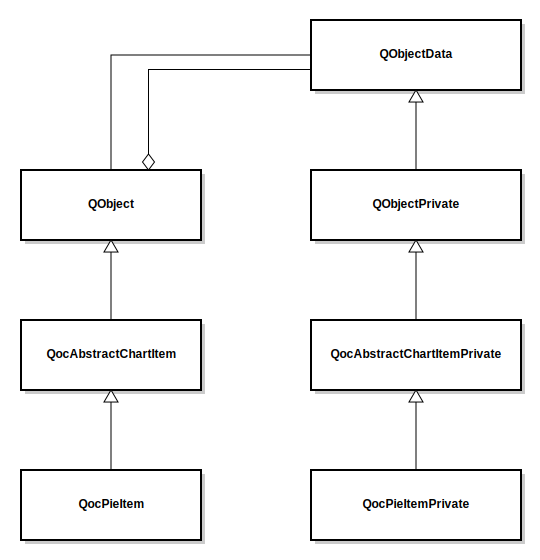
\includegraphics[scale=0.6]{dpointer.png}
\end{figure}

\subsection{Dostęp do uchwytów i ciał}
Optymalizacja opisana w~poprzednim punkcie skutkuje jednak powstaniem pewnego efektu ubocznego.
Wskaźniki do uchwytu i~ciała mają teraz typy klas znajdujących się na szczycie hierarchii dziedziczenia. Dostęp do metod klas pochodnych wymaga rzutowania w~dół. 
Problem ten rozwiązano za pomocą czterech makrodefinicji opisanych w~tabelce~\ref{tab:makra}.


\begin{table}[h]\footnotesize
  	\caption{Makrodefinicje}
	\label{tab:makra}
	\begin{tabular}{|c|c|c|}
	\hline
	Miejsce wykorzystania & Uchwyt & Ciało\\
	\hline
	Nagłówek & Q\_DECLARE\_PRIVATE & Q\_DECLARE\_PUBLIC\\
	\hline
	Początek metody & Q\_D & Q\_Q\\
	\hline
	\end{tabular}
\end{table}

\begin{thebibliography}{}
\bibitem[1]{meyers}
,,50 efektywnych sposobów na udoskonalenie Twoich programów'', Scott Meyers, strona 154, 2004, wydawnictwo Helion, ISBN: 83-7361-345-5


\end{thebibliography}
\end{document}
